\documentclass{article}
\usepackage{graphicx} % Required for inserting images
\usepackage[a4paper, left=3cm, right=2cm, top=3cm, bottom=2cm]{geometry}
\usepackage{setspace}

\usepackage{subcaption}
\title{Relatório: Sistema Fuzzy para Cálculo de Obesidade}
\author{
    Thiago Monteiro Tinonin \\
    \and
    Angelo Gabriel Vasconcelos Baptista \\
    \and
    Juan Caio Paronitti Galera \\
}
\date{Março 2025}

\begin{document}

\maketitle

\section{Variáveis}

Neste sitema foram utilizadas duas variáveis de entrada, a primeira sendo "comer" com as categorias "pouco", "razoável" e "bastante", e a segunda sendo "atividade", com as categorias "baixa", "média" e "alta". Temos como variável de saída "peso" tendo como categoria "leve", "medio", "pesado".

\section{Regras}

Foram definidas as seguintes regras para o sistema:

\begin{itemize}
  \item SE "comer bastante" E "atividade baixa" ENTÃO "ficara pesado"
  \item SE "comer pouco" ENTÃO "ficara leve"
  \item SE "comer razoavel" E "atividade média" ENTÃO "ficara médio"
  \item SE "comer bastante" E "atividade alta" ENTÃO "ficara médio"
  \item SE "comer bastante" E "atividade média" ENTÃO "ficara pesado"
\end{itemize}

\section{Saídas de funções de pertinência}

Foram gerados gráficos com base nas funções de pertinência, onde foram análisadas a sensibilidade entre variáveis de entrada e saída.

\begin{itemize}
  \item comer: 6 (equivale a um consumo de 600kcal)
  \item atividade: 7 (equivale a um nível de atividade física média/alta)
\end{itemize}

\begin{figure}[h!]
  \centering
  \begin{subfigure}[b]{0.4\linewidth}
    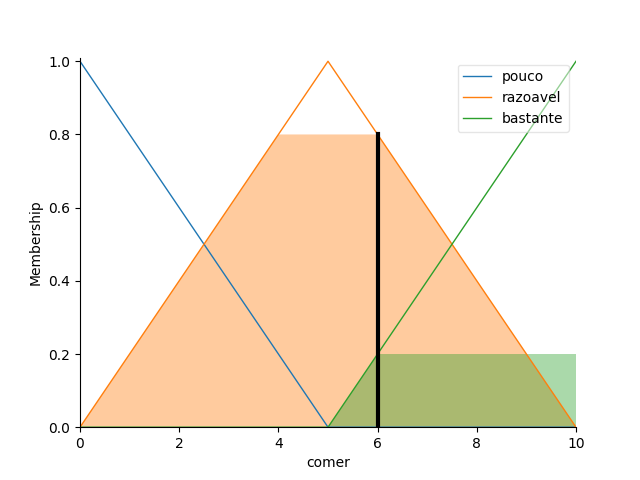
\includegraphics[width=\linewidth]{./images/comer-razoavel.png}
    \caption{Variavel comer}
  \end{subfigure}
  \begin{subfigure}[b]{0.4\linewidth}
    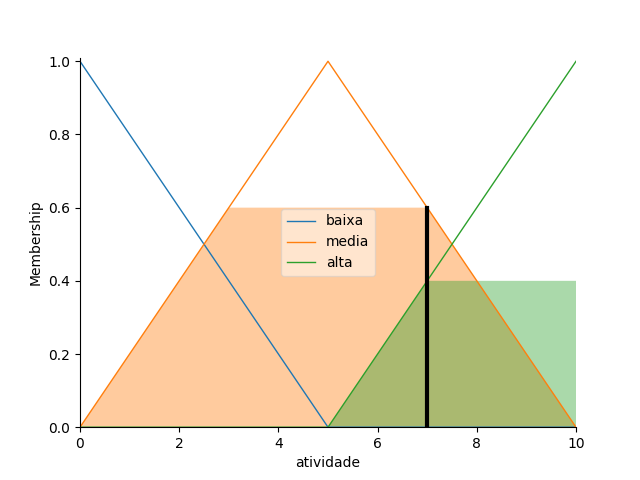
\includegraphics[width=\linewidth]{./images/atividade-media-alta.png}
    \caption{Variavel atividade}
  \end{subfigure}
  \caption{Grafícos de função de pertinência triângular de variáveis de entrada}
  \label{fig:triangular-1}
\end{figure}

\begin{figure}[h!]
  \centering
  \begin{subfigure}[b]{0.4\linewidth}
    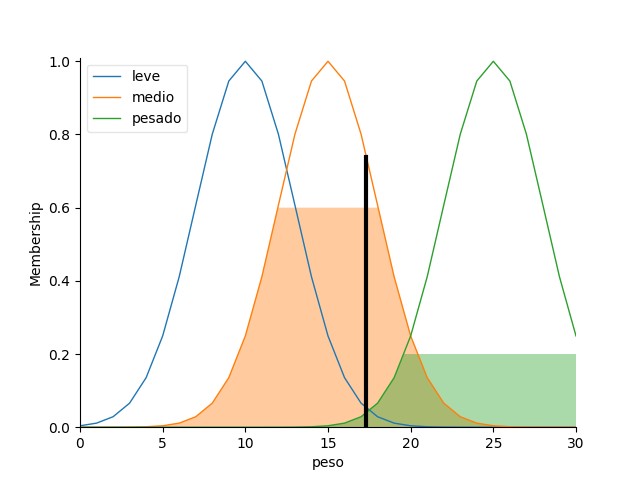
\includegraphics[width=\linewidth]{./images/peso-medio.png}
    \caption{Gaussiana}
  \end{subfigure}
  \begin{subfigure}[b]{0.4\linewidth}
    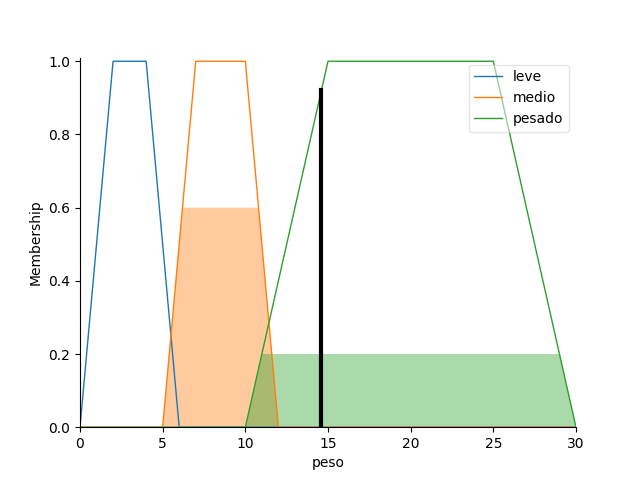
\includegraphics[width=\linewidth]{./images/peso-medio-trap.png}
    \caption{Trapezoidal}
  \end{subfigure}
  \caption{Grafícos de de saída Gaussiana e Trapezoidal}
  \label{fig:saida-1}
\end{figure}

\begin{itemize}
  \item comer: 10 (equivale a um consumo de 1000kcal)
  \item atividade: 2 (equivale a um nível de atividade física baixa)
\end{itemize}

\begin{figure}[h!]
  \centering
  \begin{subfigure}[b]{0.4\linewidth}
    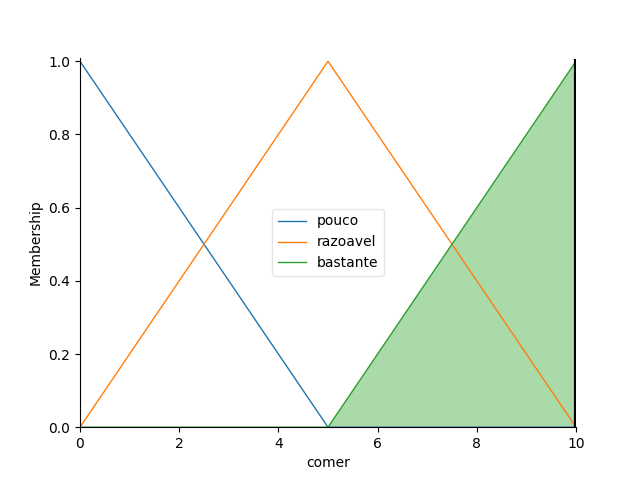
\includegraphics[width=\linewidth]{./images/comer-alto.png}
    \caption{Variavel comer}
  \end{subfigure}
  \begin{subfigure}[b]{0.4\linewidth}
    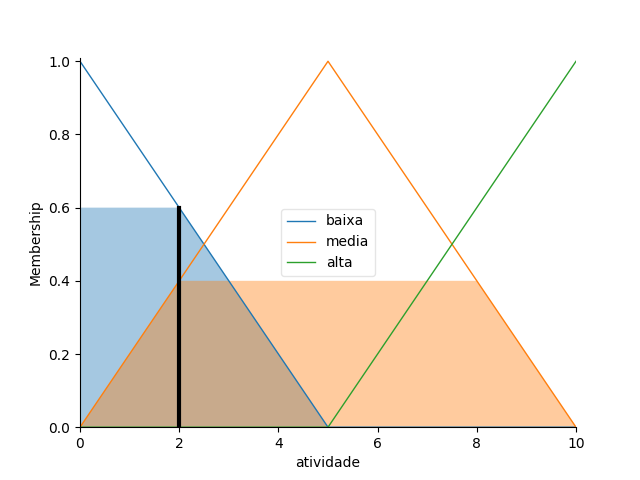
\includegraphics[width=\linewidth]{./images/atividade-baixa.png}
    \caption{Variavel atividade}
  \end{subfigure}
  \caption{Grafícos de função de pertinência triângular de variáveis de entrada}
  \label{fig:triangular-2}
\end{figure}

\begin{figure}[h!]
  \centering
  \begin{subfigure}[b]{0.4\linewidth}
    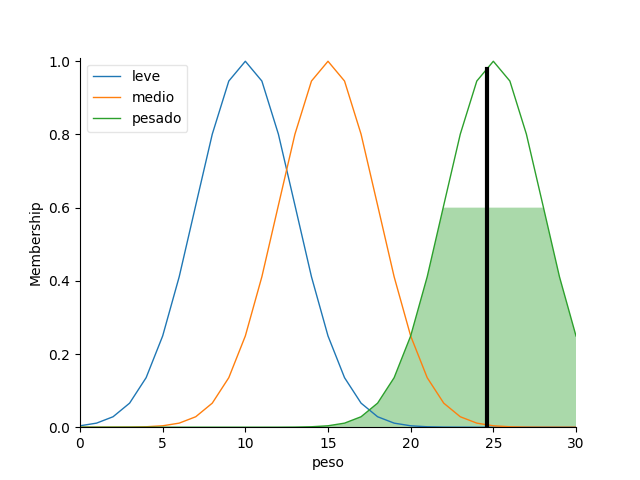
\includegraphics[width=\linewidth]{./images/peso-pesado-gauss.png}
    \caption{Gaussiana}
  \end{subfigure}
  \begin{subfigure}[b]{0.4\linewidth}
    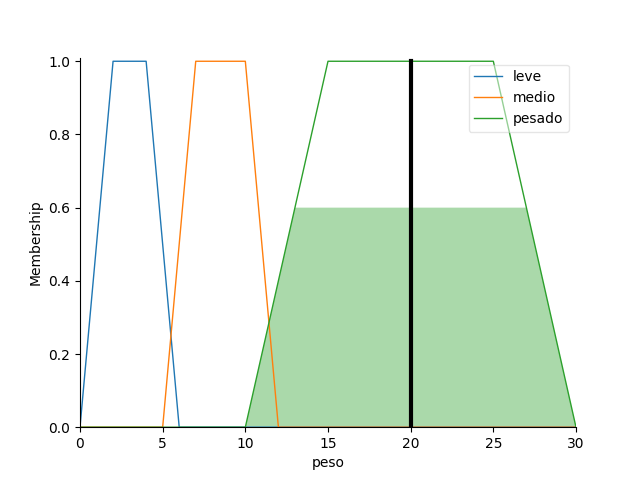
\includegraphics[width=\linewidth]{./images/peso-pesado.png}
    \caption{Trapezoidal}
  \end{subfigure}
  \caption{Grafícos de de saída Gaussiana e Trapezoidal}
  \label{fig:saida-2}
\end{figure}

\section{Conclusão}

Resolvendo este problema, foi concluido que a lógica \textit{Fuzzy} é extremamente poderosa para tratar de conceitos vagos, uma vez que as variaveis de entrada e saída do problema estejam bem definidas e com regras consistentes entre sí. Um dos desafios encontrados foi definir o conjunto de domínio para as varíaveis de funções de pertinência, porém os mesmos foram definidos após traçar-mos uma escala para melhor visualizar os valores nos gráficos, como o valor 10 em "atividade" representa 1000kcal.

\end{document}
